\begin{document}

% Lecture Notes: Hidden Markov Models for Sequence Modeling and Pattern Mining

\section{Introduction to Sequence Modeling}

A fundamental task in bioinformatics is genome annotation: deciphering the functional elements within a vast, unlabelled chunk of newly sequenced DNA. While we can search for known deterministic patterns—such as the ``ATG'' start codon for protein-coding genes—this approach is generally insufficient. Deterministic sequences occur frequently by chance in large genomes, leading to high false-positive rates. Furthermore, biological data is inherently noisy due to natural variation, evolutionary mutations, and sequencing errors. 

To effectively extract biological signals from this noise, we rely on probabilistic generative models. Unlike simple sequence profiles or motifs, which assume a fixed pattern length, advanced probabilistic models can handle variable-length functional regions, such as entire genes with differing numbers of exons, or regulatory regions like CpG islands. 

\subsection{Goals of Sequence Modeling}
By modeling DNA sequences probabilistically, we achieve three primary objectives:
\begin{itemize}
    \item \textbf{Generative Simulation}: The ability to emit or generate random DNA sequences of a specific type (e.g., simulating promoters) that preserve the statistical properties of that type, even if they do not identically match any known sequence.
    \item \textbf{Sequence Recognition}: The ability to analyze an unlabelled sequence and infer the hidden state (e.g., coding vs. non-coding) that was most likely to have generated the observed nucleotides.
    \item \textbf{Feature Learning}: The ability to train generative models on large datasets to automatically learn the distinguishing sequence characteristics of different genomic states.
\end{itemize}

\section{Markov Chains and Hidden Markov Models (HMMs)}

To handle probabilistic sequence modeling with variable lengths, we utilize frameworks built upon stochastic processes originally formulated by the Russian mathematician Andrey Markov. 

\subsection{Markov Chains}

A Markov Chain is a model that transitions between different states over time, where each state is directly observable. 

\begin{important}
\textbf{Markov Chain}: A probabilistic model defined as a triplet $(Q, p, A)$, where:
\begin{itemize}
    \item $Q$ is a finite set of states, directly corresponding to the observable alphabet $\Sigma$.
    \item $p$ is a vector of initial state probabilities.
    \item $A$ is the matrix of state transition probabilities, where $a_{kl} = P(x_i = l \mid x_{i-1} = k)$ for states $k, l \in Q$.
\end{itemize}
\textbf{Key Property (Memorylessness)}: The probability of transitioning to the next state depends \textit{only} on the current state, independent of the history of previous states: 
\[ P(x_i \mid x_{i-1}, \dots, x_1) = P(x_i \mid x_{i-1}) \]
\end{important}

For a Markov Chain, the probability of observing a specific sequence $x$ of length $L$ is simply the product of the initial probability and all subsequent transitions:
\begin{equation}
P(x) = P(x_1) \times \prod_{i=2}^{L} P(x_i \mid x_{i-1})
\label{eq:markov_prob}
\end{equation}

\subsection{Hidden Markov Models}

In many real-world scenarios, the underlying state dictating the behavior of a system cannot be directly observed. For example, we observe weather (sun, rain, snow), but the underlying season (summer, winter) that generates those weather probabilities is hidden. In genomics, we observe a sequence of nucleotides (A, C, G, T), but the functional state (promoter, exon, intron) generating those nucleotides is hidden.

\begin{important}
\textbf{Hidden Markov Model (HMM)}: A probabilistic model defined as a 5-tuple $(Q, V, p, A, E)$, where:
\begin{itemize}
    \item $Q$ is a finite set of $N$ \textit{hidden states} $q_n$.
    \item $V$ is a finite set of $M$ \textit{observable symbols} $v_m$.
    \item $p$ is a vector of initial state probabilities.
    \item $A$ is an $N \times N$ state transition probability matrix, where $a_{kl} = P(\pi_i = l \mid \pi_{i-1} = k)$.
    \item $E$ is an $N \times M$ emission probability matrix, where $e_k(v_m) = P(x_i = v_m \mid \pi_i = k)$.
\end{itemize}
\end{important}

\sta Both state transitions and symbol emissions are memoryless. The emission probability depends solely on the current hidden state and remains constant over time. We use Bayes' rule to infer the hidden state $\pi_i = k$ given the observed symbol $x_i$.

% [IMAGE: Side-by-side comparison. Left side shows a Markov Chain of weather (Sun, Clouds, Rain, Snow) transitioning directly between each other. Right side shows an HMM where hidden states (Summer, Winter) transition between each other, and each hidden state emits observable weather symbols with specific probabilities.]

\subsection{Example Models}

\textbf{Example: The Dishonest Casino} \\
A hypothetical casino utilizes two dice: a Fair die ($D_F$) and a Loaded die ($D_L$). The player cannot see which die the dealer is using (the hidden state).
\begin{itemize}
    \item \textbf{States ($Q$)}: Fair ($F$), Loaded ($L$).
    \item \textbf{Observables ($V$)}: Dice rolls $\{1, 2, 3, 4, 5, 6\}$.
    \item \textbf{Transitions ($A$)}: The dealer switches dice on average once every 20 turns. Thus, $P(F \to F) = 0.95$, $P(F \to L) = 0.05$, $P(L \to L) = 0.95$, $P(L \to F) = 0.05$.
    \item \textbf{Emissions ($E$)}: 
    \begin{itemize}
        \item Fair die: $P(1) = P(2) = P(3) = P(4) = P(5) = P(6) = \frac{1}{6}$
        \item Loaded die: $P(6) = \frac{1}{2}$, and $P(1) = \dots = P(5) = \frac{1}{10}$.
    \end{itemize}
\end{itemize}

\begin{center}
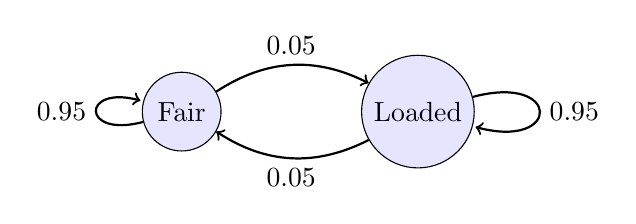
\begin{tikzpicture}[node distance=3cm, state/.style={circle, draw, minimum size=1cm, fill=blue!10}]
    \node[state] (F) {Fair};
    \node[state, right of=F] (L) {Loaded};
    
    \path[->, thick]
    (F) edge [loop left] node {0.95} (F)
    (F) edge [bend left] node[above] {0.05} (L)
    (L) edge [loop right] node {0.95} (L)
    (L) edge [bend left] node[below] {0.05} (F);
\end{tikzpicture}
\end{center}

\textbf{Example: The Dishonest Genome}\\
Similar to the casino, a genome might randomly transition between human DNA and integrated viral DNA. The observable alphabet is $\{A, C, G, T\}$. Viral DNA and Human DNA will have distinct emission probabilities for these nucleotides (e.g., varying GC-content).

\section{The Six Algorithmic Settings for HMMs}

To fully utilize an HMM, we must solve several distinct computational problems. These can be grouped into evaluation (scoring), decoding (finding the path), and learning (training), applied either to a single optimal path or to all possible paths.

\begin{table}[h]
\centering
\begin{tabularx}{\textwidth}{l X X}
\toprule
\textbf{Task} & \textbf{One Path (Optimal)} & \textbf{All Paths (Summed)} \\
\midrule
\textbf{Evaluation} & 1. Scoring $x$ over the optimal path. & 2. Scoring $x$ over all paths (Forward algorithm). \\
\textbf{Decoding} & 3. Finding the best state sequence (Viterbi algorithm). & 4. Probabilistic label per position (Posterior decoding). \\
\textbf{Learning} & 5a. Supervised MLE (if labels known). \newline 5b. Viterbi training (if labels unknown). & 6. Baum-Welch / Expectation-Maximization (if labels unknown). \\
\bottomrule
\end{tabularx}
\caption{The six algorithmic settings for handling HMMs in sequence analysis.}
\end{table}

\section{Evaluation: Scoring a Sequence}

\subsection{Scoring One Path (Joint Probability)}
Given a known sequence of observations $x$ and a specifically assumed hidden path $\pi$, the joint probability $P(x, \pi)$ is simply the product of the probabilities of all transitions and emissions along that exact route.

\[ P(x, \pi) = P(x \mid \pi) P(\pi) = p(\pi_1) e_{\pi_1}(x_1) \prod_{i=1}^{N-1} a_{\pi_i \pi_{i+1}} e_{\pi_{i+1}}(x_{i+1}) \]

\textbf{Example:} Evaluating the Dishonest Casino. \\
For sequence $x = 1, 2, 1, 5, 6, 2, 1, 6, 2, 4$, assume the path $\pi = \text{all-Fair}$.
\[ P(x, \text{all-Fair}) = \frac{1}{2} \times \left(\frac{1}{6}\right)^{10} \times (0.95)^9 = 5.2 \times 10^{-9} \]
If we instead test $\pi = \text{all-Loaded}$:
\[ P(x, \text{all-Loaded}) = \frac{1}{2} \times \left(\frac{1}{10}\right)^8 \times \left(\frac{1}{2}\right)^2 \times (0.95)^9 = 7.9 \times 10^{-10} \]
This output is 6.59 times more likely to be generated by a completely Fair die than a completely Loaded die. 

\sta \textit{Why are these probabilities so minuscule?} Because there are millions of possible hidden paths and outcomes. When dealing with real genomes, joint probabilities approach zero rapidly, necessitating the use of log-scores to prevent computational underflow.

\subsection{Scoring All Paths (The Forward Algorithm)}
In reality, a specific output $x$ could be generated by many different hidden paths. To find the total probability $P(x)$ that the model generated the sequence, we must sum the joint probabilities over an exponential number of possible paths. 

\[ P(x) = \sum_{\pi} P(x, \pi) = \sum_{\pi} P(x \mid \pi) P(\pi) \]

We compute this efficiently in $O(K^2 N)$ time using dynamic programming via the \textbf{Forward Algorithm}. We define the forward probability $f_k(i)$ as the probability of emitting the prefix $x_1 \dots x_i$ and ending up in state $\pi_i = k$.

\begin{important}
\textbf{Forward Algorithm (Iterative Step)}:
\[ f_k(i) = e_k(x_i) \times \sum_j \left[ a_{jk} f_j(i-1) \right] \]
where we sum over all possible previous states $j$.
\end{important}

\section{Decoding: Finding the Hidden States}

Given only the observed emissions $x$, how do we infer the hidden states? We have two primary methods depending on whether we want the single best global path, or the best sequence of local states.

\subsection{Finding the Optimal Path: The Viterbi Algorithm}

The \textbf{Viterbi algorithm} finds the single most likely path $\pi^*$ that maximizes the joint probability $P(x, \pi)$. It relies on the principle of optimal substructure: the best path through a given state at step $i$ is composed of the best path to a state at step $i-1$, followed by the optimal transition to the current state.

\begin{important}
\textbf{Viterbi Algorithm}: Let $V_k(i)$ be the probability of the most likely path generating sequence $x_1 \dots x_i$ and ending in state $k$.
\begin{itemize}
    \item \textbf{Initialization}: $V_0(0) = 1$; $V_k(0) = 0$ for all $k > 0$.
    \item \textbf{Iteration}: $V_k(i) = e_k(x_i) \times \max_j \left[ a_{jk} V_j(i-1) \right]$
    \item \textbf{Termination}: $P(x, \pi^*) = \max_k V_k(N)$
\end{itemize}
\end{important}

\begin{minted}{python}
# [pseudocode]
def viterbi(observations, states, initial_p, trans_p, emit_p):
    V = [{}]
    path = {}
    
    # Initialization
    for state in states:
        V[state] = initial_p[state] * emit_p[state][observations]
        path[state] = [state]
        
    # Iteration
    for t in range(1, len(observations)):
        V.append({})
        new_path = {}
        for current_state in states:
            # Find the max probability from previous states
            (max_prob, best_prev_state) = max(
                (V[t-1][prev_state] * trans_p[prev_state][current_state] * emit_p[current_state][observations[t]], prev_state)
                for prev_state in states
            )
            V[t][current_state] = max_prob
            new_path[current_state] = path[best_prev_state] + [current_state]
        path = new_path
        
    # Termination
    (max_prob, final_state) = max((V[-1][state], state) for state in states)
    return path[final_state], max_prob
\end{minted}

The Viterbi algorithm works almost identically to sequence alignment dynamic programming. In each column (representing an observation), we look back at the entire previous column (all possible previous states). We multiply the probability of being in the previous state by the transition probability to the current state, and take the maximum. Finally, we multiply by the emission probability of the current state. We keep a "traceback pointer" to the chosen previous state so that at the end of the sequence, we can trace back from the highest final probability to recover the optimal path.

\subsection{Posterior Decoding: The Forward-Backward Algorithm}

The Viterbi path provides the single best sequence, but it ignores the probability mass of all other valid paths. For genome annotation, we often want the most likely state for a \textit{specific position} $i$, averaged over all possible paths. This requires \textbf{Posterior Decoding}.

To do this, we need the probability of the sequence up to $i$ (Forward algorithm) and the probability of the sequence from $i+1$ to the end (Backward algorithm).

\begin{important}
\textbf{Backward Algorithm}: Let $b_k(i)$ be the probability of emitting the suffix $x_{i+1} \dots x_N$ given that the state at step $i$ is $k$.
\begin{itemize}
    \item \textbf{Initialization}: $b_k(N) = a_{k0}$ (transition to end state) for all $k$.
    \item \textbf{Iteration}: $b_k(i) = \sum_l \left[ e_l(x_{i+1}) a_{kl} b_l(i+1) \right]$
\end{itemize}
\end{important}

Once we have computed the matrices for both $f_k(i)$ and $b_k(i)$, we can calculate the posterior probability of being in state $k$ at position $i$ given the entire sequence $x$:
\begin{equation}
P(\pi_i = k \mid x) = \frac{f_k(i) b_k(i)}{P(x)}
\end{equation}

By choosing the state $k$ that maximizes this probability at each position $i$, we generate a sequence of labels. 
\sta Note that the resulting sequence of states from posterior decoding might be an \textit{invalid path} (e.g., predicting a transition between two states that has a transition probability of 0). However, it provides the most statistically refined measure of the local state at every single nucleotide position.

\section{Learning: Training an HMM}

Before we can use an HMM to decode a genome, we must estimate its parameters: transition probabilities $a_{kl}$ and emission probabilities $e_k(b)$.

\subsection{Supervised Learning (Known Labels)}
If we possess labeled training data (e.g., a chromosome where CpG islands have already been experimentally verified), learning is straightforward via Maximum Likelihood Estimation (MLE). We simply count occurrences:
\[ a_{kl} = \frac{A_{kl}}{\sum_i A_{ki}} \quad \text{and} \quad e_k(b) = \frac{E_k(b)}{\sum_c E_k(c)} \]
where $A_{kl}$ is the absolute count of transitions from $k$ to $l$, and $E_k(b)$ is the count of state $k$ emitting symbol $b$.

\sta \textbf{The Danger of Zero Probabilities}: Given limited data, strict MLE often results in probabilities of 0 for rare events. In an HMM, a single zero probability destroys the entire product chain, making a path computationally impossible. We resolve this by adding \textbf{pseudocounts} to all raw counts before normalizing. 
\[ A_{kl} = (\text{observed count}) + r_{kl} \]

\subsection{Unsupervised Learning (Unknown Labels)}
Often, we have unlabelled data (e.g., a newly sequenced species). We start with an initial guess for the parameters and iteratively improve them.

\textbf{Viterbi Training (Hard Assignments)}:
\begin{enumerate}
    \item Guess initial parameters.
    \item Run Viterbi decoding to find the optimal path $\pi^*$.
    \item Treat $\pi^*$ as the true labels to calculate new MLE parameters (supervised learning step).
    \item Iterate until convergence.
\end{enumerate}

\textbf{Baum-Welch Algorithm / Expectation-Maximization (Soft Assignments)}:
Viterbi training is flawed because it relies on a single path. Baum-Welch training considers the weighted contribution of \textit{all paths}.
\begin{enumerate}
    \item \textbf{Initialization}: Guess parameters.
    \item \textbf{E-Step (Expectation)}: Run the Forward and Backward algorithms. Estimate the expected number of transitions and emissions probabilistically across all possible paths.
    \item \textbf{M-Step (Maximization)}: Calculate new maximum likelihood parameters based on the probabilistic expectations derived in the E-step.
    \item Iterate until the overall likelihood $P(x \mid \theta)$ ceases to improve significantly.
\end{enumerate}
This expectation-maximization (EM) process guarantees that the log-likelihood of the model will increase with each iteration, guaranteeing convergence to at least a local optimum.

\section{Increasing State Space to Encode Memory}

By mathematical definition, Markov models are memoryless. The current state determines the emission and transition probabilities, utterly independent of the prior path. 

However, biology often requires memory. For example, to accurately model a CpG island, we must know that the current nucleotide is G \textit{and} the previous nucleotide was C. How can we count di-nucleotide frequencies in a memoryless system?

\textbf{Solution}: We expand the state space.
To remember a previous nucleotide, we embed that memory into the identity of the current state itself. Instead of having just 2 states (CpG-rich vs Background), we create 8 states:
\begin{itemize}
    \item CpG-rich states: $A_+, C_+, G_+, T_+$
    \item Background states: $A_-, C_-, G_-, T_-$
\end{itemize}

% [IMAGE: Graph showing 8 nodes instead of 2. The four '+' nodes represent nucleotides emitted inside a CpG island, and the four '-' nodes represent nucleotides emitted in background DNA. Transition arrows between C+ and G+ are given very high weight to simulate the biological prevalence of CpG dinucleotides.]

If the system emits a `C` while in a CpG-island, it enters the $C_+$ state. From $C_+$, we can manually assign a highly inflated transition probability to $G_+$, accurately simulating the di-nucleotide frequency of CpG islands while strictly adhering to the memoryless rules of the Markov framework. Similarly, in protein-coding gene models, expanding state space allows us to track reading frames (codons) across spliced introns by having $E_0, E_1, E_2$ and $I_0, I_1, I_2$ states.

\end{document}